\documentclass{article}
\usepackage{amsmath, amsthm, amssymb, booktabs, hyperref, graphicx, float, esint, xcolor, subcaption}
\setlength{\abovedisplayskip}{0pt}
\setlength{\belowdisplayskip}{0pt}
\setlength{\abovedisplayshortskip}{0pt}
\setlength{\belowdisplayshortskip}{0pt}

\newcommand{\vr}{\vec{r}}
\newcommand{\vOmega}{\vec{\Omega}}
\newcommand{\vO}{\vec{\Omega}}
\newcommand{\bra}{\left\langle}
\newcommand{\ket}{\right\rangle}
\newcommand{\vdiv}{\vec{\nabla} \cdot}
\newcommand{\vgrad}{\vec{\nabla}}
\newcommand{\vbeta}{\vec{\beta} }
\newcommand{\pdx}{\frac{\partial}{\partial x}}
\newcommand{\pdy}{\frac{\partial}{\partial y}}
\newcommand{\pdz}{\frac{\partial}{\partial z}}
\newcommand{\intrrr}{\int d^3 r \,}
\newcommand{\intrr}{\int d^2 r \,}
\newcommand{\dEdphi}{\partial_\phi E \,}
\newcommand{\dEdp}{\partial_p E \,}
\newcommand{\dBdphi}{\partial_\phi B \,}
\newcommand{\dBdp}{\partial_p B \,}
\newcommand{\adj}{\phi^\dag}
\newcommand{\surf}{\int_{\partial V}}
\newcommand{\vn}{\vec{n}}
\newcommand{\Edd}{\mathbf{E}}
\newcommand{\BEdd}{\mathbf{B}}
\newcommand{\sigt}{\sigma_t}
\newcommand{\sigs}{\sigma_s}
\newcommand{\siga}{\sigma_a}
\newcommand{\isigt}{c}
\newcommand{\angSource}{q_\Omega}
\newcommand{\scalSource}{q}
\newcommand{\angResp}{r_\Omega}
\newcommand{\scalResp}{r}
\newcommand{\qoi}{QoI}

\begin{document}
\begin{center}
{\large Thesis Proposal }\\
Ian Halvic, Texas A\&M University, NUEN \\
Adjoint-based sensitivity for radiation transport using an Eddington tensor formulation \\
\end{center}

\tableofcontents

%%%%%%%%%%%%%%%%%%%%%%%%%%%%%%%%%%%%%%%%%%%%%%%%%%%%%%%%%%%%%%%%%%%%%%%%%%%%%%%%%%%%%%%%%%%%%%%%%%%%
\section{Introduction}
%%%%%%%%%%%%%%%%%%%%%%%%%%%%%%%%%%%%%%%%%%%%%%%%%%%%%%%%%%%%%%%%%%%%%%%%%%%%%%%%%%%%%%%%%%%%%%%%%%%%
\begin{itemize}
\item predictive science -> need for UQ and sensitivity [Nat'l Aca]
\item adjoint methods have been dev. to provide sensi coefs; [Marchuk]; mathematical technique based on inner products; why useful: many sources -> many direct solve (forward) but only 1 forward and 1 adjoint for same answers
\item adjoint methods also used for time-dep problems [find refs, fluid flow, Sandia]. in time-dep problem, the forward time-dep solution needs to be stored for later use in the adjoitn formalism [put that proof with a simple linear operator du/dt + Au = q in appendix of thesis]
\item time-dep transport would require very large memory usage to store forward solution because rad transport is a 6D (high dimensional phase space problem at every time step)
\item idea investigated in this these: use of an low-order representation for rad transport: VET. 
\item: setting of the study: single group (one-speed) steady state transport 
\end{itemize}

{\color{red}[IWH: Notation Questions? At what point does it become acceptable to drop the independent variables ($(\vr,\vO,E)$ and such) on the flux and cross section terms? Should I be using uppercase $\Sigma$ instead of $\sigma$ for the cross-sections in this context? I know that the uppercase is more technically correct for neutrons, but we seemed to always just use lower cases when talking.]}

%%%%%%%----------------------------------------------------------------------------------------------
\subsection{Steady-state one-group neutron transport equation}
%%%%%%%----------------------------------------------------------------------------------------------

The time dependent neutron transport equation without fission is given to be 
\begin{equation}
\frac{1}{v(E)} \frac{\partial}{\partial t}\psi + \vO \cdot \vgrad \psi + \sigt(\vr,E,t) \psi = \int_{4 \pi} d \Omega^\prime \, \int_0^\infty dE^\prime \sigs(\vr,E^\prime \to E, \vO^\prime \to \vO) \psi + S(\vr,E,\vO,t) 
\end{equation}
{\color{red}[IWH: Add boundary condition (numbering? should the BC have its own EQ number, or be lumped with the main). Introduction of terms in the TE here. Definition of relevant volume $V$ and boundary $\Gamma$]}
\\ \\
{\color{red}[IWH: Present why the TE in its complete form is unwieldy. Transition into the simplifying approximations below.]}
The first simplifying approximation to be made is that scattering is isotropic, allowing the use of an energy differential scattering cross section $\sigs(\vr,E^\prime \to E)$. This also allows for the use of the scalar flux $\phi$ in the scattering term.
\begin{equation}
\frac{1}{v(E)} \frac{\partial}{\partial t}\psi + \vO \cdot \vgrad \psi + \sigt(\vr,E,t) \psi = \frac{\phi}{4 \pi} \int_0^\infty dE^\prime \sigs(\vr,E^\prime \to E) + S(\vr,E,\vO,t) 
\end{equation}
 \\ \\
For practicality, the energy dependence is discritized into a finite number of energy groups. Let each each energy group be denoted by the subscript $g \in (1,G)$. 
\begin{equation}
\frac{1}{v(E)} \frac{\partial}{\partial t}\psi_g + \vO \cdot \vgrad \psi_g + \sigt(\vr,E,t) \psi_g = \frac{1}{4 \pi} \sum_{g^\prime=1}^G  \Sigma_{s,g^\prime}(\vr) \phi_{g^\prime} + S_g(\vr,\vO,t) 
\end{equation}
In the above equation, scattering terms for $g^\prime \neq q$ are inscattering terms, and act as a source term for a given energy group. Making the assumption that the fixed source term $S_g$ is isotropic, allows the generation of a total source term $q$.
\begin{equation}
\begin{split}
\frac{1}{v(E)} \frac{\partial}{\partial t}\psi_g &+ \vO \cdot \vgrad \psi_g + \sigt(\vr,E,t) \psi_g \\
&= \frac{1}{4 \pi} \sum_{g^\prime=1}^G  \Sigma_{s,g^\prime}(\vr) \phi_{g^\prime} + S_g(\vr,\vO,t) \\
&= \frac{1}{4 \pi} \Sigma_{s,g^\prime}(\vr) \phi_{g}
+ \frac{1}{4 \pi} \sum_{g^\prime=1}^G  \Sigma_{s,g^\prime}(\vr) \phi_{g^\prime} + S_g(\vr,\vO,t)  \quad :g^\prime \neq g\\
&= \frac{1}{4 \pi} \Sigma_{s,g^\prime}(\vr) \phi_{g}
+ \frac{q_g}{4 \pi}\
\end{split}
\end{equation}
{\color{red}[IWH: NEED TO SWITCH TO STEADY STATE AT SOME POINT! I think I need guidance on how to transition from the time dependent equation to the steady state, to transition into the steady state Sn and VET formulations we have primarily been working with]}

{\color{red}[IWH: I feel like I need to go back through the literature and cite more for the simplifying assumptions.]}

%%%%%%%----------------------------------------------------------------------------------------------
\subsection{Quantity of interest and their sensitivities}
%%%%%%%----------------------------------------------------------------------------------------------

{\color{red}[IWH: This I really just need to go back into the literature, (particularly National Research Council) and present why obtaining the sensitivity is of importance for verification/validation/UQ. What are sour of important things for me to look at here?]}

solution of a simulation is not necessarily the sought after answer. -- QoI which depends on the solution itself

%----------------------------------------------------------------------------------------------
\subsubsection{Quantity of interest, response function and inner products}
%----------------------------------------------------------------------------------------------

Given $\psi(\vr,\vO)$ the solution of the one-group steady-state transport (Eq.~\eqref{eq:transport_eq}), one typically seeks a QoI
defined as

\[
\qoi =  \int_V dV \int_{4 \pi} d \vO \,  r(\vr, \vO) \psi(\vr, \vO)
\]

explain $r$ (and already mention $r$ will be switched to $q^\dag$ later) and then introduce inner products

For this paper, two inner products are defined both using $\bra \bullet , \bullet \ket$ notation. These two inner-products are for use with angular dependent and scalar functions, so the use of a single notation should be unambiguous.
\begin{equation}
\bra f , g \ket_{V \times \mathcal{S}_2}  = \int_V dV \int_{4 \pi} d \vO \,  f(\vr, \vO)g(\vr, \vO)
\end{equation}

\begin{equation}
\bra f(\vr) , g(\vr) \ket  = \int_V dV \,  f(\vr)g(\vr)
\end{equation}

when unambiguous, say you drop the ...

\begin{equation}
( f , g )_{\partial V \times \mathcal{S}_2}  = \int_{\partial V} dS \int_{4 \pi} d \vO \, \vO \cdot \vn(\vr) \, f(\vr, \vO)g(\vr, \vO)
\end{equation}
\begin{equation}
( f , g )_{\pm}   = \int_{\partial V} dS \int_{\vO \cdot \vn \gtrless 0} d\vO \,  \vO \cdot \vn(\vr) \, f(\vr, \vO)g(\vr, \vO)
\end{equation}


[define QoI]
\begin{equation}
\label{QoIDef}
\qoi = \bra \psi(\vr,\vO), \angResp(\vr,\vO) \ket = \bra \phi(\vr) , \scalResp(\vr) \ket
\end{equation}

%----------------------------------------------------------------------------------------------
\subsubsection{Sensitivity to Inputs}
%----------------------------------------------------------------------------------------------
sensitivity to what? parameter of the equation .... sigma's, q ....

A hurdle in utilizing the transport equation numerically to make real world predictions is that none of the system's parameters ($\sigt$, $sigs$, $q$, and $\psi^{inc}$) are never known exactly.


%%%%%%%----------------------------------------------------------------------------------------------
\subsection{Adjoint sensitivity (Alternate writeup, Marchuk Cite)}
%%%%%%%----------------------------------------------------------------------------------------------

Adjoint operators can provide a useful tool for sensitivity calculations. Using inner product notation $\bra \bullet , \bullet \ket$, consider the system of interest $\mathbf{A}f = q$. Call this this the forward system, with forward operator $\mathbf{A}$. Considering valid test function $\varphi$, that adjoint operator $\mathbf{A^\dag}$ is defined as $\bra \mathbf{A} f, \varphi \ket = \bra f, \mathbf{A^\dag} \varphi \ket $. For differential operators, derivation of $\mathbf{A^\dag}$ generally relies on Green's first identity (integration by parts), typically resulting in boundary terms not show here. Using the response function corresponding to the desired $\qoi$, the adjoint system can be constructed as $\mathbf{A^\dag} \varphi=r$ leading to an alternate expression of the $\qoi$ using the adjoint solution $\varphi$.
\begin{equation}
\label{genAdjQoI}
\qoi = \bra f, r \ket = \bra s , \varphi \ket + bc
\end{equation} 
From the above, it follows that a first order approximation to the change in the quantity of interest based on perturbations to the initial system, including perturbation to the forward operator $\delta \mathbf{A}$ and forward source $\delta q$, can be expressed in the form shown in Eq.~\eqref{genAdjSens} \cite{Marchuk}.
\begin{equation}
\label{genAdjSens}
\delta \qoi \approx \bra \delta q - \delta \mathbf{A} f , \varphi \ket 
\end{equation}
The advantage of the above expression for $\delta \qoi$ is that two solves, one for the forward and another for the adjoint, can be used to approximate the sensitivity for a variety $\delta \mathbf{A}$ and $\delta q$.

 
%%%%%%%%%%%%%%%%%%%%%%%%%%%%%%%%%%%%%%%%%%%%%%%%%%%%%%%%%%%%%%%%%%%%%%%%%%%%%%%%%%%%%%%%%%%%%%%%%%%%
\section{Discrete Ordinates (Sn) Transport}
%%%%%%%%%%%%%%%%%%%%%%%%%%%%%%%%%%%%%%%%%%%%%%%%%%%%%%%%%%%%%%%%%%%%%%%%%%%%%%%%%%%%%%%%%%%%%%%%%%%%
With the energy discretization performed, the transport equation system has become a system of $G$ equations of the form shown in equation \ref{1gTE}, coupled by the inscattering terms wrapped up in the source term $q$.
\begin{equation}
\label{1gTE}
\vO \cdot \vgrad \psi + \sigt \psi = \frac{\sigs}{4 \pi} \phi + \frac{q}{4 \pi} \quad \vr \in V , \forall \vO \in \mathcal{S}_2
\end{equation}
\begin{equation}
\psi(\vr,\vO) = \psi^{\text{inc}}(\vr,\vO) \quad \vr \in \partial V^{-} = \{ \vr \in \partial V, \text{ s.t. }, \vO \cdot \vec{n}(\vr) < 0\}
\end{equation}
The unknowns in the above include the angular flux $\psi=\psi(\vr,\vO)$ and the scalar flux $\phi=\phi(\vr)$. A discrete ordinates (Sn) method can be used to discretize the angular variable. Using a an gular quadrature with $D$ directions $\vO_d$, the transport equation is solved along each direction:
\begin{equation}
\label{1gTE}
\vO_d \cdot \vgrad \psi_d + \sigt \psi_d = \frac{\sigs}{4 \pi} \phi + \frac{q}{4 \pi} \quad \vr \in V , \forall d\in [1,D]
\end{equation}
%
The scalar flux can be computed from the angular flux as follows
\[
\phi(\vr) \approx \sum_{d=1}^D w_d \psi_d(\vr)
\] 
where $\psi_d(\vr) = \psi(\vr, \vO_d)$ and $w_d$ is a quadrature weight. This leads to a coupled system of $D$ equations of the form shown in equation \cite{SnFwd}, where the system is coupled through the scalar flux term.
%
\begin{equation}
\label{snFwd}
\vO \cdot \vgrad \psi + \sigt \psi = \frac{\sigs}{4 \pi} \phi + q
\end{equation}
\begin{equation}
\psi(\vr) = \psi^{\text{out}}(\vr) \quad \vr \in \Gamma, Sn \cdot \vec{n} < 0
\end{equation}

{\color{red}[Is the Sn form just discrete ordinates, or does it require full decomposition into the discretized FEM form?]}

%%%%%%%----------------------------------------------------------------------------------------------
\subsection{Adjoint Sn formulation}
%%%%%%%----------------------------------------------------------------------------------------------
[in MS thesis, put demonstration]\\

In a fairly straight forward application of the adjoint method previously shown, the adjoint equation which corresponds to the Sn transport formulation with response $\angResp$ is
\begin{equation}
\label{snAdj}
- \vO \cdot \vgrad \psi^\dag + \sigt \psi^\dag = \frac{\sigs}{4 \pi} \phi^\dag + \angResp
\end{equation}
%
\begin{equation}
\psi^\dag(\vr,\vO) = \psi^{\dag \text{out}}(\vr,\vO) \quad \vr \in \Gamma, \vO \cdot \vec{n} > 0
\end{equation}
where the definition of the adjoint scalar flux $\phi^\dag$ is analogous to the forward definition. It is worth noting that the SN adjoint equation is in the form of a transport equation, only with the direction of travel reversed ($\vO \to -\vO)$. This often allows for forward Sn transport solvers to be easily adapted to solving the Sn adjoint system. Once the adjoint solution is obtained, the corresponding QoI can be calculated with a simple inner product with the forward source term, as follows from equation \ref{adjGeneral2}. 
%
\begin{equation}
\label{snAdjQoI}
QoI = \bra \psi^\dag , \angSource \ket - \int d^2 r \, \int d  \Omega \, \psi^\dag \psi ( \vO \cdot \vec{n} )
\end{equation}
%
The surface interval in \ref{snAdjQoI} can be split into incoming and outgoing flux integrals, which are handled by the forward and adjoint boundary conditions respectively. 
%
\begin{equation}
QoI = \bra \psi^\dag , q \ket - \int d^2 r \, \int_{\vO \cdot \vec{n} >0} d  \Omega \, \psi^\dag \psi ( \vO \cdot \vec{n} ) - \int d^2 r \, \int_{\vO \cdot \vec{n} <0} d  \Omega \, \psi^\dag \psi ( \vO \cdot \vec{n} )
\end{equation}

%%%%%%%----------------------------------------------------------------------------------------------
\subsection{Sn Transport Adjoint Sensitivity}
%%%%%%%----------------------------------------------------------------------------------------------

Now consider perturbations to our system. Specifically perturbations of $\delta \sigt$, $\delta \sigs$, and $\delta q$ to the total cross section, scattering cross section and angular source term respectively. In addition, the incident angular flux is also perturbed by $delta \psi^{inc}$. These perturbations result is a perturbed solution to the Sn-transport equation $\psi_p$. Using this $\delta$ notation, the perturbed Sn-equation is shown in \ref{snPert}
\begin{equation}
\label{snPert}
\vO \cdot \vgrad \psi_p + \left( \sigt + \delta \sigt \right) \psi_p = \frac{\left( \sigs + \delta \sigs \right)}{4 \pi} \phi_p + \left( \angSource + \delta \angSource \right)
\end{equation}
\begin{equation}
\psi_p(\vr,\vO) = \psi^{\text{inc}}(\vr,\vO) + \delta \psi^{\text{inc}}(\vr,\vO)\quad \vr \in \Gamma
\end{equation}
This perturbation may result in a change to the QoI, now given by $QOI_p=\bra \psi_p , \angResp \ket$. Retaining the unperturbed adjoint equation given in \ref{snAdj} and using a first order approximation of the perturbed Sn transport equation \ref{snPert}, the perturbed QoI can be represented as an inner product not dependent on the perturbed forward solution.
\begin{equation}
\label{snSens}
\begin{split}
QoI_p &=\bra \psi_p , \angResp \ket \\
&=\bra \psi_p , - \vO \cdot \vgrad \psi^\dag + \sigt \psi^\dag - \frac{\sigs}{4 \pi} \phi^\dag  \ket \\
&= \bra  \vO \cdot \vgrad \psi_p + \sigt \psi_p - \frac{\sigs}{4 \pi} \phi_p , \psi^\dag  \ket - \int_{\Gamma} \int_{\Omega} \psi_p \psi^\dag \vO \cdot \vec{n}\\
&= \bra  \scalSource - \delta \sigt \psi + \frac{\delta\sigs}{4 \pi} \phi + \delta \scalSource , \psi^\dag  \ket - \int_{\Gamma} \int_{\Omega} \psi_p \psi^\dag \vO \cdot \vec{n}\\
\end{split}
\end{equation}
Subtraction of the unperturbed $QoI$ expression in equation \ref{snAdjQoI} supplies a final equation for computing the change in $QoI$ using only the system perturbations and the unperturbed forward and adjoint solutions, removing the need to solve the perturbed forward equation.
\begin{equation}
\delta QoI_p = \bra - \delta \sigt \psi + \frac{\delta\sigs}{4 \pi} \phi + \delta \scalSource , \psi^\dag  \ket - \int_{\Gamma} \int_{\Omega} \delta \psi \psi^\dag \vO \cdot \vec{n}\\
\end{equation}

%%%%%%%%%%%%%%%%%%%%%%%%%%%%%%%%%%%%%%%%%%%%%%%%%%%%%%%%%%%%%%%%%%%%%%%%%%%%%%%%%%%%%%%%%%%%%%%%%%%%
\section{VET formulation}
%%%%%%%%%%%%%%%%%%%%%%%%%%%%%%%%%%%%%%%%%%%%%%%%%%%%%%%%%%%%%%%%%%%%%%%%%%%%%%%%%%%%%%%%%%%%%%%%%%%%

%%%%%%%----------------------------------------------------------------------------------------------
\subsection{Motivation} 
%%%%%%%----------------------------------------------------------------------------------------------

While the Sn adjoint sensitivity formulation given by \ref{snSens} provides a first-order accurate method to determine the sensitivity to multiple perturbation scenarios using only a single forward and adjoint transport solve, it can quickly run into technical limitations. Specifically for even a one-group time independent system, all solutions to the forward and adjoint system in space and angle must be stored for retrieval later. For a spatially 3-dimensional system, this translates to storing descritized data across 5-dimensions.


%%%%%%%----------------------------------------------------------------------------------------------
\subsection{VET Formulation}
%%%%%%%----------------------------------------------------------------------------------------------

The "Variable Eddington Tensor" (VET) formulation shows promise of reducing the memory requirements when using the adjoint method for sensitivity. To begin the formulation, the steady state transport equation is expanded to the scalar and first angular moment by application of the $\int d \Omega$ and $\int d \Omega \, \vO$ operators to equation \ref{1gTE}, respectively. Using the notation
\begin{equation}
\phi=\int d\Omega \, \psi( \vO )
,\quad
\vec{J}= \int d\Omega \, \vO \psi( \vO )
\end{equation}
the zero-th and first angular moment transport equations are
\begin{equation}
\label{0am}
\vdiv \vec{J} + \sigt \phi = \sigs \phi + \scalSource
\end{equation}
\begin{equation}
\label{1am}
\vdiv \left(  \int d\Omega \vO \vO \psi \right) + \sigt \vec{J} =0 
\end{equation}
The Eddington Tensor $\Edd$ is then introduced as a simplifying approximation relating the second angular moment term in equation \ref{1am} to the scalar flux. 
\begin{equation}
\label{EddDef}
\Edd=\frac{\int d\Omega \vO \vO \psi}{\phi}
\end{equation}
The inclusion of the Eddington tensor allow equation \ref{1am} to be expressed as $\sigt \vec{J} = - \vdiv \Edd \phi$. Using this as a definition of $\vec{J}$ allows us to convert \ref{0am} to the form shown in \ref{VEFForm}, which only has the scalar flux as an unknown. The substitution $\siga = \sigt-\sigs$ was used.
\begin{equation}
\label{VEFForm}
- \vdiv \left( \frac{1}{\sigt}\vdiv \Edd \phi \right) + \siga \phi = \scalSource
\end{equation}
The known incident flux can be used to generate a suitable boundary condition using a "Boundary Eddington Factor" $B$ \cite{Miften}.
\begin{equation}
\frac{1}{\sigma_{t} } \vec{\nabla} \cdot \left(\Edd \phi \right)  = - 2J^- - B \phi \quad \vr \in \Gamma
\end{equation}
\begin{equation}
B= \frac{\int_{4 \pi} d\Omega \, \left| \Omega_i n_i \right | \psi}{\int_{4\pi} d\Omega \, \psi} \quad \vr \in \Gamma
\end{equation}

%%%%%%%----------------------------------------------------------------------------------------------
\subsection{Adjoint VET formulation}
%%%%%%%----------------------------------------------------------------------------------------------

The VET formulation necessitates a reformulation of our adjoint. As shown in \ref{adjForm}, the double divergence term present in the forward equation contributes to a double gradient term in the adjoint equation.
\begin{equation}
\label{adjForm}
- \Edd : \left( \vgrad \left( \frac{1}{\sigt}\vgrad \phi^\dag \right) \right) + \siga \phi^\dag = \scalResp
\end{equation}
For reasons that will become apparent during sensitivity calculations, the boundary condition chosen for the adjoint equation is given in \ref{adjVETBC}. Unlike for Sn formulation, the VET adjoint equation does not take the form of a VET transport equation.
\begin{equation}
\label{adjVETBC}
\Edd \cdot \frac{1}{\sigma_{t} } \vec{\nabla} \phi^\dag  = - 2J^{\dag +} - B \phi^\dag \quad \vr \in \Gamma
\end{equation}
To obtain the QoI using this formulation, begin with the typical QoI definition, relocate operators to the forward to substitute the forward source, and apply boundary conditions.
\begin{equation}
\label{VETQoIAdjUnpDeriv}
\begin{split}
QoI=&\bra \phi , \scalResp \ket \\
=&\bra \phi , - \Edd : \left( \vgrad \isigt \vgrad \phi^\dag \right) + \siga \phi^\dag \ket \\
=& \bra - \vdiv \isigt \vdiv \left( \Edd \phi \right) + \siga \phi, \phi^\dag \ket 
- \int_\Gamma d^2 r \, \phi \left( \Edd \cdot \isigt \vgrad \phi^\dag \right) \cdot \vec{n}  \\ 
&+ \int_\Gamma d^2 r \, \phi^\dag \left(  \isigt \vgrad \Edd \phi \right) \cdot \vec{n} \\
=&\bra \scalSource , \phi^\dag \ket 
- \int_\Gamma d^2 r \, \phi \left( - 2J^{\dag +} - B \phi^\dag \right) \cdot \vec{n} + \int_\Gamma d^2 r \, \phi^\dag \left( - 2J^- - B \phi  \right) \cdot \vec{n}
\end{split}
\end{equation}
The boundary Eddington terms negate and yield a relatively compact form for the QoI
\begin{equation}
\label{VETQoIAdj}
QoI=\bra \scalSource , \phi^\dag \ket 
+ \int_\Gamma d^2 r \, 2  \left( \phi J^{\dag +}  - \phi^\dag J^- \right) \cdot \vec{n}
\end{equation}

%%%%%%%----------------------------------------------------------------------------------------------
\subsection{VET adjoint sensitivity}
%%%%%%%----------------------------------------------------------------------------------------------

As was done in the Sn transport formulation, once again consider perturbations to the system parameters. However, in contrast to the Sn case, the assumption is also made that the Eddington factor remains unperturbed under these system perturbations. For brevity, the substitution of $\isigt = \sigt^{-1}$ was also made.
\begin{equation}
\label{VEFPert}
- \vdiv \left((\isigt + \delta \isigt)\vdiv \Edd \phi_p \right) + (\siga + \delta \siga)\phi_p = \scalSource + \delta \scalSource
\end{equation}
\begin{equation}
(\isigt + \delta \isigt) \vec{\nabla} \cdot \left(\Edd \phi_p \right)  = - 2J_p^- - B \phi_p \quad \vr \in \Gamma
\end{equation}
The usual adjoint process is performed, starting with the QoI definition using the perturbed solution and response. 
\begin{equation}
\label{VETSensDeriv}
\begin{split}
\qoi=&\bra \phi_p , \scalResp \ket \\
=&\bra \phi_p , - \Edd : \left( \vgrad \isigt \vgrad \phi^\dag \right) + \siga \phi^\dag \ket \\
=& \bra - \vdiv \isigt \vdiv \left( \Edd \phi_p \right) + \siga \phi_p, \phi^\dag \ket 
- \int_\Gamma d^2 r \, \phi_p \left( \Edd \cdot \isigt \vgrad \phi^\dag \right) \cdot \vec{n}  \\ 
&+ \int_\Gamma d^2 r \, \phi^\dag \left(  \isigt \vgrad \Edd \phi_p \right) \cdot \vec{n} \\
\end{split}
\end{equation}
A first order perturbation approximation of equation \ref{VEFPert} can be used to substitute into the sensitivity equation \ref{VETSensDeriv}, yielding a form independ of the perturbed forward solution.
\begin{equation}
\label{QoIVETAdjNoBC}
\begin{split}
\qoi =& \bra \scalSource + \delta \scalSource + \vdiv \delta \isigt \vdiv \left( \Edd \phi \right) - \delta \siga \phi, \phi^\dag \ket - \int_\Gamma d^2 r \, \phi_p \left( \Edd \cdot \isigt \vgrad \phi^\dag \right) \cdot \vec{n} 
\\ &+ \int_\Gamma d^2 r \, \phi^\dag \left(  \isigt \vdiv \Edd \phi_p \right) \cdot \vec{n} 
\end{split}
\end{equation}
The first surface term can be dealt with readily using the adjoint boundary condition. For the second surface term, a first order approximation of the perturbed forward boundary condition is used for substitution.
\begin{equation}
\label{QoIVETAdj}
\begin{split}
\qoi =& \bra \scalSource + \delta \scalSource + \vdiv \delta \isigt \vdiv \left( \Edd \phi \right) - \delta \siga \phi, \phi^\dag \ket - \int_\Gamma d^2 r \, \phi_p \left( - 2J^{\dag +} - B \phi^\dag \right) \cdot \vec{n} 
\\ &+ \int_\Gamma d^2 r \, \phi^\dag \left( - 2J_p^- - B \phi_p - \delta \isigt \vdiv \Edd \phi \right) \cdot \vec{n} 
\end{split}
\end{equation}
Subtract the adjoint $\qoi$ formulation from equation \ref{VETQoIAdj} to obtain the sensitivity expression for the adjoint VET formulation.
\begin{equation}
\label{SensVETAdjNoBC}
\begin{split}
\delta \qoi =& \bra \delta \scalSource + \vdiv \delta \isigt \vdiv \left( \Edd \phi \right) - \delta \siga \phi, \phi^\dag \ket + \int_\Gamma d^2 r \, 2  \left( \delta \phi J^{\dag +}  - \phi^\dag \delta J^- \right) \cdot \vec{n}
\\ &- \int_\Gamma d^2 r \,  \phi^\dag \left( \delta \isigt \vdiv \Edd \phi \right) \cdot \vec{n} 
\end{split}
\end{equation}


%%%%%%%----------------------------------------------------------------------------------------------
\subsection{Error from unperturbed Eddington assumption}
%%%%%%%----------------------------------------------------------------------------------------------

Beyond the first order approximation common to adjoint formulations, the VET sensitivity formulation also made the assumption that the Eddington tensor remained unperturbed under perturbations of the other parameters. To observe the terms that were dropped in this approximation, consider a reformulation of the perturbed forward equation, this time introducing $\delta \Edd$ and $\delta  B$ terms. 
\begin{equation}
\label{VEFPerEdd}
- \vdiv \left((\isigt + \delta \isigt)\vdiv (\Edd + \delta \Edd) \phi_p \right) + (\siga + \delta \siga)\phi_p = \scalSource + \delta \scalSource
\end{equation}
\begin{equation}
(\isigt + \delta \isigt) \vec{\nabla} \cdot \left((\Edd + \delta \Edd) \phi_p \right)  = - 2J_p^- - (\BEdd +\delta \BEdd) \phi_p \quad \vr \in \Gamma
\end{equation}
The above can be substituted into equation \ref{VETSensDeriv} to yield an expanded $\qoi$ equation, including the Eddington perturbation terms
\begin{equation}
\label{QoIVETAdjNoBCEdd}
\begin{split}
\qoi =& \bra \scalSource + \delta \scalSource + \vdiv \delta \isigt \vdiv \left( \Edd \phi \right) + \vdiv \isigt \vdiv \left( \delta \Edd \phi \right) - \delta \siga \phi, \phi^\dag \ket \\
&- \int_\Gamma d^2 r \, \phi_p \left( \Edd \cdot \isigt \vgrad \phi^\dag \right) \cdot \vec{n} 
+ \int_\Gamma d^2 r \, \phi^\dag \left(  \isigt \vdiv \Edd \phi_p \right) \cdot \vec{n} 
\end{split}
\end{equation}
The boundary condition for the perturbed forward solution takes on a slightly more complex form, as the additional $\delta \Edd$ and $\delta \BEdd$ terms come into play, but the derivation of the sensitivity proceeds similarly to the case ignoring Eddington perturbations.
\begin{equation}
\label{QoIVETAdjEdd}
\begin{split}
\delta \qoi =& \bra \delta \scalSource + \vdiv \delta \isigt \vdiv \left( \Edd \phi \right) + \vdiv \isigt \vdiv \left( \delta \Edd \phi \right) - \delta \siga \phi, \phi^\dag \ket \\
&+ \int_\Gamma d^2 r \, 2  \left( \delta \phi J^{\dag +}  - \phi^\dag \delta J^- \right) \cdot \vec{n}
- \int_\Gamma d^2 r \,  \phi^\dag \left( \delta \isigt \vdiv \Edd \phi \right) \cdot \vec{n}
\\
&- \int_\Gamma d^2 r \,  \phi^\dag \left( \isigt \vdiv \delta \Edd \phi \right) \cdot \vec{n}
- \int_\Gamma d^2 r \,  \phi^\dag \phi \delta \BEdd \cdot \vec{n}
\end{split}
\end{equation} 
Comparing the above formulation with the unperturbed Eddington case shows that the perms lost by the Unperturbed Eddington assumption are 
\begin{equation}
\label{EddErr}
 \bra \vdiv \isigt \vdiv \left( \delta \Edd \phi \right), \phi^\dag \ket
- \int_\Gamma d^2 r \,  \phi^\dag \left( \isigt \vdiv \delta \Edd \phi \right) \cdot \vec{n}
- \int_\Gamma d^2 r \,  \phi^\dag \phi \delta \BEdd \cdot \vec{n}
\end{equation} 

%%%%%%%%%%%%%%%%%%%%%%%%%%%%%%%%%%%%%%%%%%%%%%%%%%%%%%%%%%%%%%%%%%%%%%%%%%%%%%%%%%%%%%%%%%%%%%%%%%%%
\section{Preliminary results}
%%%%%%%%%%%%%%%%%%%%%%%%%%%%%%%%%%%%%%%%%%%%%%%%%%%%%%%%%%%%%%%%%%%%%%%%%%%%%%%%%%%%%%%%%%%%%%%%%%%%

{\color{red}[IWH: Explain what I am looking at (VET adjoint versus Sn adjoint, versus multiple forward solves). I need to touch up these graphs (do them in Matlab, not Excel). Introduce the FEM parameters used.]}

%%%%%%%----------------------------------------------------------------------------------------------
\subsection{Homogeneous initial system, Uniform Perturbations}
%%%%%%%----------------------------------------------------------------------------------------------
The first test case consisted of a 1D homogeneous system, with a volumetric source throughout. Solutions were obtained using a 200 element FEM mesh. Three systems of varying initial cross sections $\sigt$ and $\sigs$ were tested. Perturbations in $\sigt$, $\sigs$, and $\scalSource$ to the system were made uniformly, resulting in the perturbed system remaining homogeneous.

\begin{figure}[H]
\label{HomoPertt}
\centering
\begin{subfigure}{.5\textwidth}
  \centering
  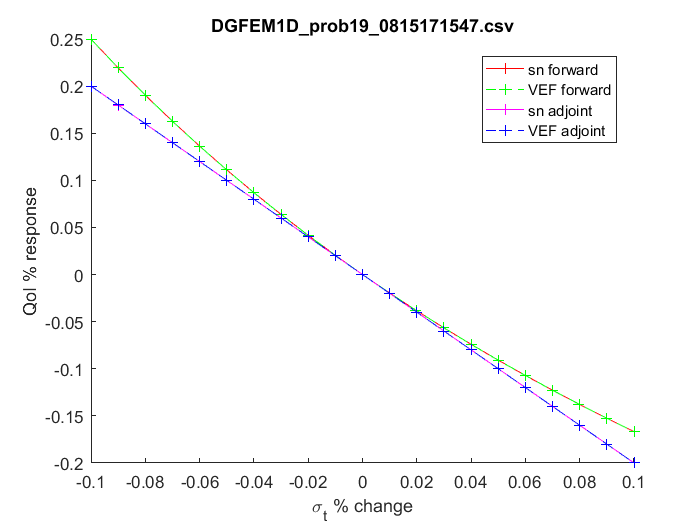
\includegraphics[width=.8\linewidth]{figures/19sigtSens.png}
  \caption{$\sigt=2$, $\sigs=1$}
  \label{fig:sfig1}
\end{subfigure}%
\begin{subfigure}{.5\textwidth}
  \centering
  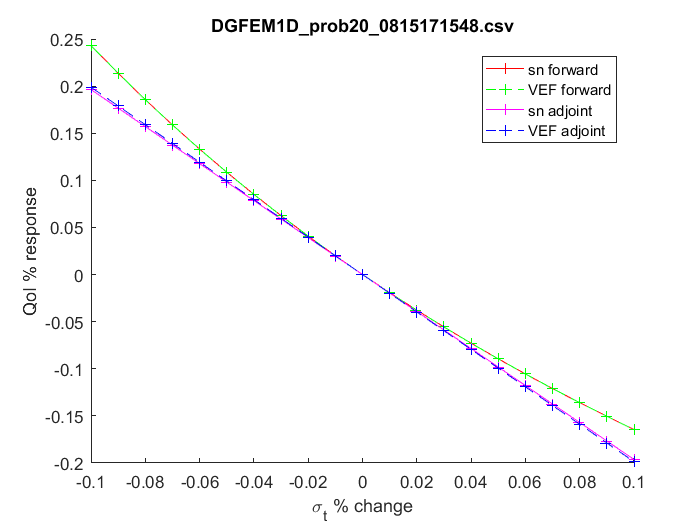
\includegraphics[width=.8\linewidth]{figures/20sigtSens.png}
  \caption{$\sigt=1$, $\sigs=0.5$}
  \label{fig:sfig2}
\end{subfigure}
\begin{subfigure}{.5\textwidth}
  \centering
  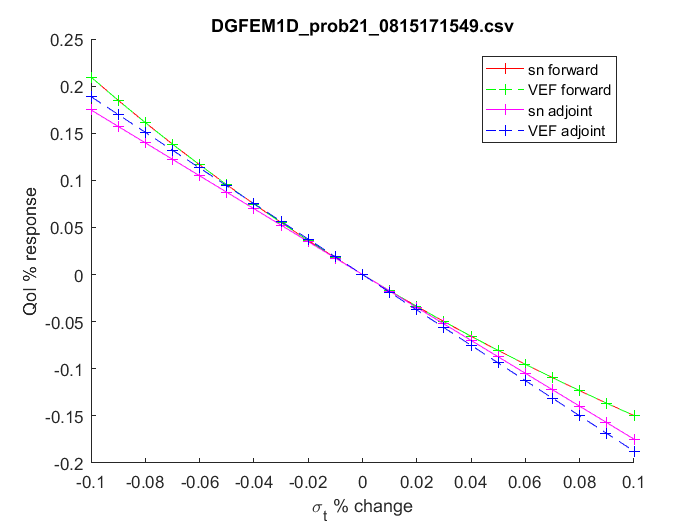
\includegraphics[width=.8\linewidth]{figures/21sigtSens.png}
  \caption{$\sigt=0.5$, $\sigs=0.25$}
  \label{fig:sfig3}
\end{subfigure}
\caption{Plots of $\sigt$ perturbation sensitivity.}
\label{fig:fig}
\end{figure}

\begin{figure}[H]
\label{HomoPerts}
\begin{subfigure}{.5\textwidth}
  \centering
  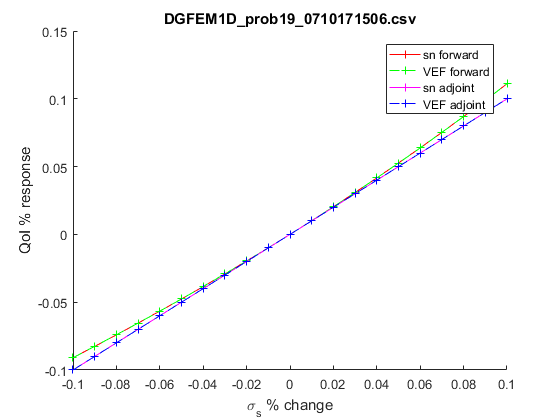
\includegraphics[width=.8\linewidth]{figures/19sigsSens.png}
  \caption{$\sigt=2$, $\sigs=1$}
  \label{fig:sfig1}
\end{subfigure}%
\begin{subfigure}{.5\textwidth}
  \centering
  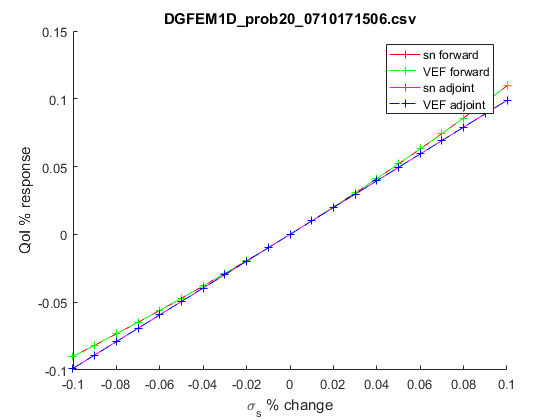
\includegraphics[width=.8\linewidth]{figures/20sigsSens.png}
  \caption{$\sigt=1$, $\sigs=0.5$}
  \label{fig:sfig2}
\end{subfigure}
\begin{subfigure}{.5\textwidth}
  \centering
  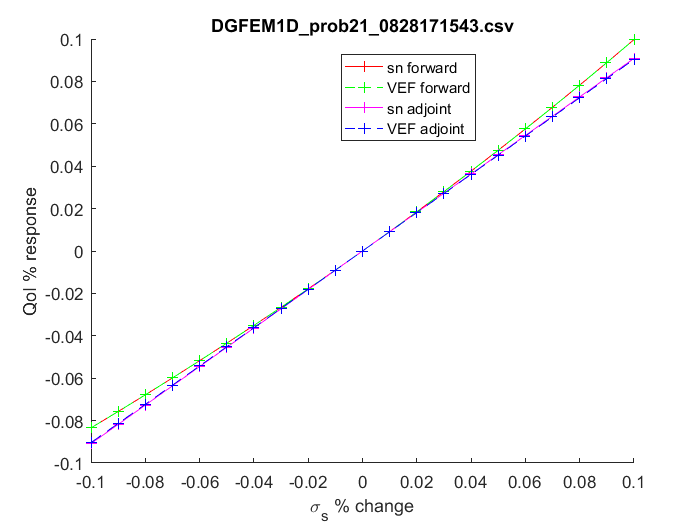
\includegraphics[width=.8\linewidth]{figures/21sigsSens.png}
  \caption{$\sigt=0.5$, $\sigs=0.25$}
  \label{fig:sfig3}
\end{subfigure}
\caption{Plots of $\sigs$ perturbation sensitivity.}
\label{fig:fig}
\end{figure}

\begin{figure}[H]
\label{HomoPertq}
\begin{subfigure}{.5\textwidth}
  \centering
  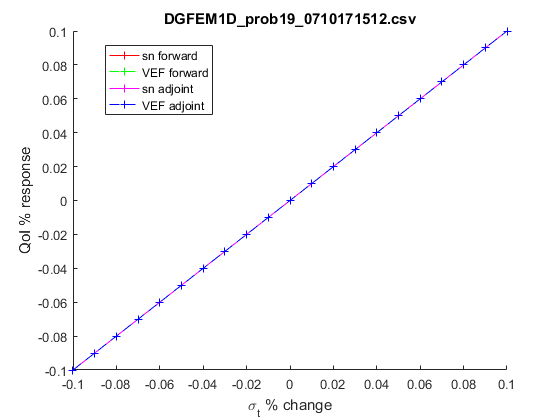
\includegraphics[width=.8\linewidth]{figures/19qSens.png}
  \caption{$\sigt=2$, $\sigs=1$}
  \label{fig:sfig1}
\end{subfigure}%
\begin{subfigure}{.5\textwidth}
  \centering
  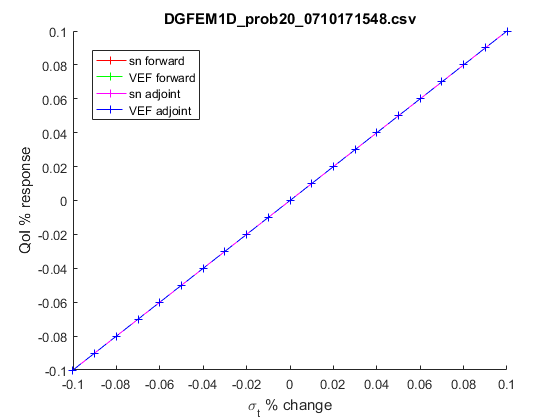
\includegraphics[width=.8\linewidth]{figures/20qSens.png}
  \caption{$\sigt=1$, $\sigs=0.5$}
  \label{fig:sfig2}
\end{subfigure}
\begin{subfigure}{.5\textwidth}
  \centering
  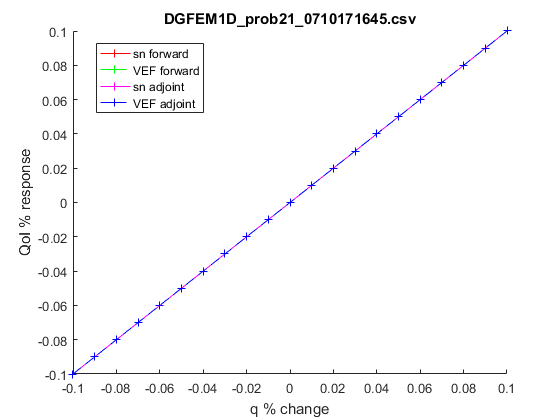
\includegraphics[width=.8\linewidth]{figures/21qSens.png}
  \caption{$\sigt=0.5$, $\sigs=0.25$}
  \label{fig:sfig3}
\end{subfigure}
\caption{Plots of source perturbation sensitivity.}
\label{fig:fig}
\end{figure}

%%%%%%%----------------------------------------------------------------------------------------------
\subsection{Homogeneous initial system, Non-Uniform Perturbations}
%%%%%%%----------------------------------------------------------------------------------------------

[Define system,  perturbations, and QoI. Vary MFP between cases.]
\begin{figure}[H]
\label{InHomoPertt}
\begin{subfigure}{.5\textwidth}
  \centering
  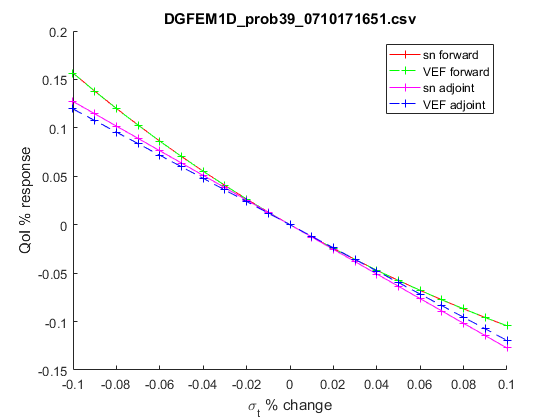
\includegraphics[width=.8\linewidth]{figures/39sigtSens.png}
  \caption{$\sigt=2$, $\sigs=1$}
  \label{fig:sfig1}
\end{subfigure}%
\begin{subfigure}{.5\textwidth}
  \centering
  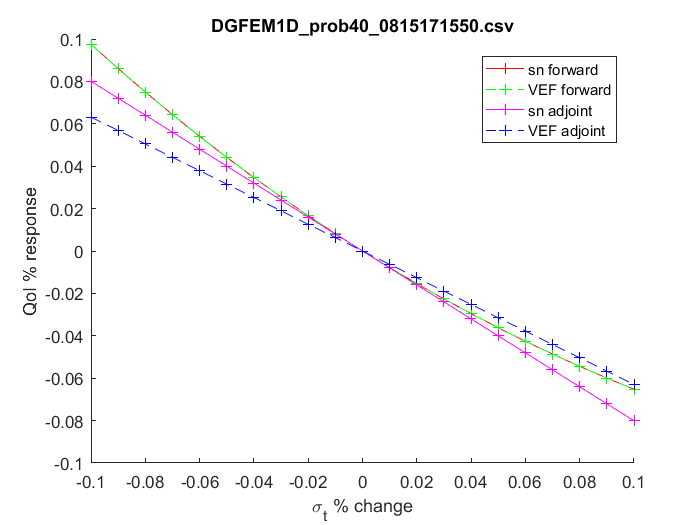
\includegraphics[width=.8\linewidth]{figures/40sigtSens.png}
  \caption{$\sigt=1$, $\sigs=0.5$}
  \label{fig:sfig2}
\end{subfigure}
\begin{subfigure}{.5\textwidth}
  \centering
  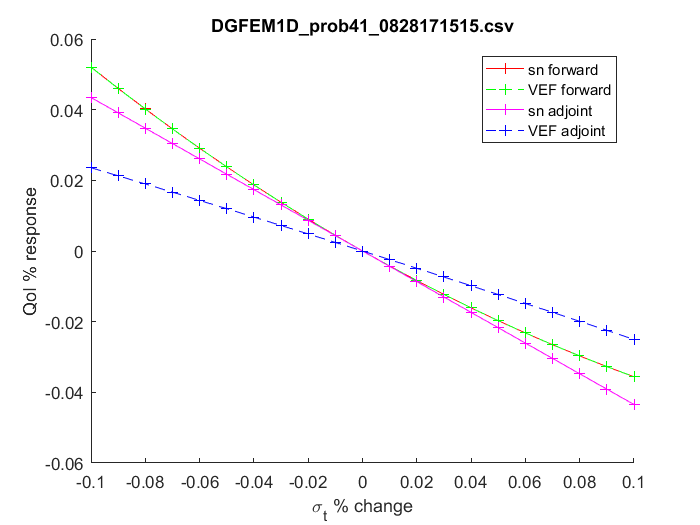
\includegraphics[width=.8\linewidth]{figures/41sigtSens.png}
  \caption{$\sigt=0.5$, $\sigs=0.25$}
  \label{fig:sfig3}
\end{subfigure}
\caption{Plots of $\sigt$ perturbation sensitivity.}
\label{fig:fig}
\end{figure}

\begin{figure}[H]
\label{InHomoPerts}
\begin{subfigure}{.5\textwidth}
  \centering
  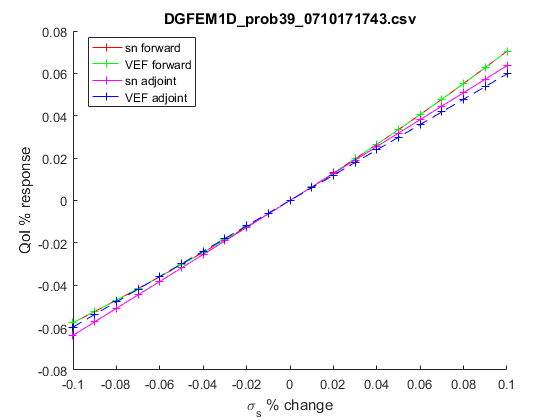
\includegraphics[width=.8\linewidth]{figures/39sigsSens.png}
  \caption{$\sigt=2$, $\sigs=1$}
  \label{fig:sfig1}
\end{subfigure}%
\begin{subfigure}{.5\textwidth}
  \centering
  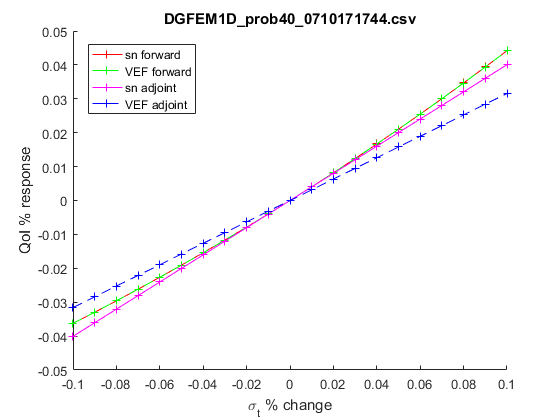
\includegraphics[width=.8\linewidth]{figures/40sigsSens.png}
  \caption{$\sigt=1$, $\sigs=0.5$}
  \label{fig:sfig2}
\end{subfigure}
\begin{subfigure}{.5\textwidth}
  \centering
  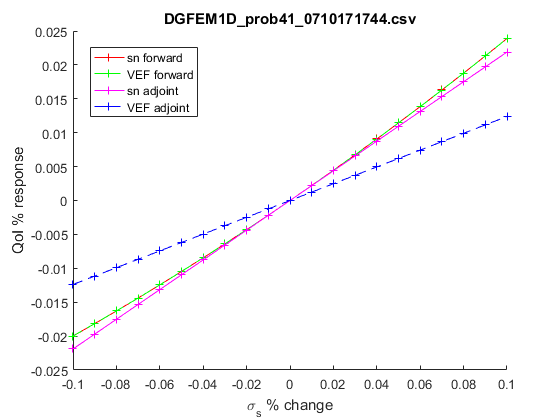
\includegraphics[width=.8\linewidth]{figures/41sigsSens.png}
  \caption{$\sigt=0.5$, $\sigs=0.25$}
  \label{fig:sfig3}
\end{subfigure}
\caption{Plots of $\sigs$ perturbation sensitivity.}
\label{fig:fig}
\end{figure}

\begin{figure}[H]
\label{InHomoPertq}
\begin{subfigure}{.5\textwidth}
  \centering
  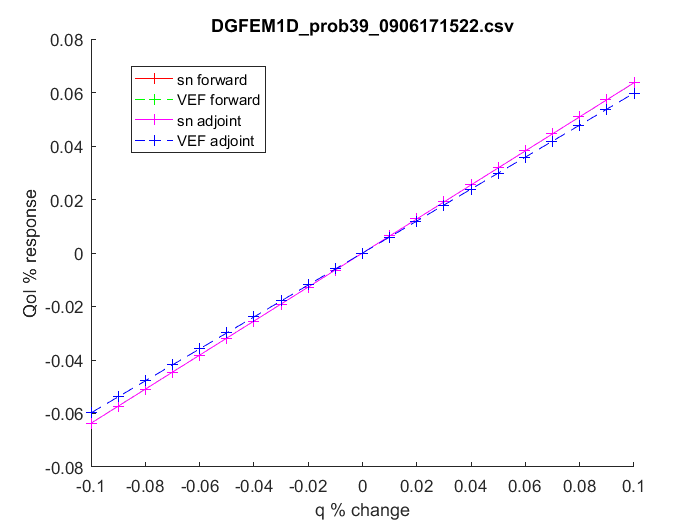
\includegraphics[width=.8\linewidth]{figures/39qSens.png}
  \caption{$\sigt=2$, $\sigs=1$}
  \label{fig:sfig1}
\end{subfigure}%
\begin{subfigure}{.5\textwidth}
  \centering
  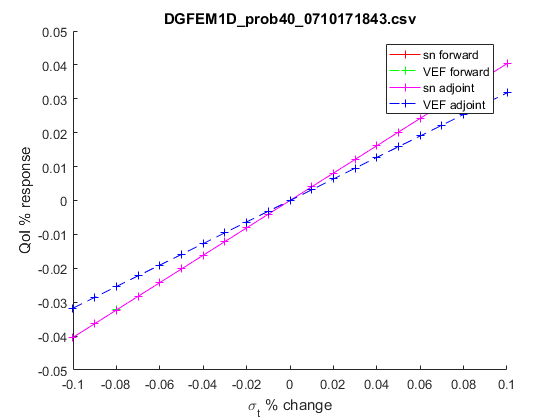
\includegraphics[width=.8\linewidth]{figures/40qSens.png}
  \caption{$\sigt=1$, $\sigs=0.5$}
  \label{fig:sfig2}
\end{subfigure}
\begin{subfigure}{.5\textwidth}
  \centering
  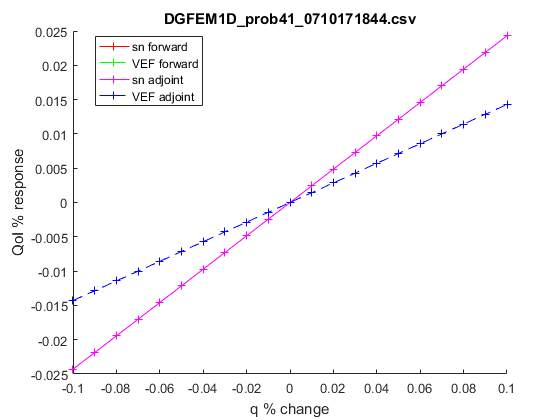
\includegraphics[width=.8\linewidth]{figures/41qSens.png}
  \caption{$\sigt=0.5$, $\sigs=0.25$}
  \label{fig:sfig3}
\end{subfigure}
\caption{Plots of source perturbation sensitivity.}
\label{fig:fig}
\end{figure}

%%%%%%%----------------------------------------------------------------------------------------------
\subsection{Streaming system}
%%%%%%%----------------------------------------------------------------------------------------------

[Define system,  perturbations, and QoI.]

%%%%%%%%%%%%%%%%%%%%%%%%%%%%%%%%%%%%%%%%%%%%%%%%%%%%%%%%%%%%%%%%%%%%%%%%%%%%%%%%%%%%%%%%%%%%%%%%%%%%%
\section{Goals}
%%%%%%%%%%%%%%%%%%%%%%%%%%%%%%%%%%%%%%%%%%%%%%%%%%%%%%%%%%%%%%%%%%%%%%%%%%%%%%%%%%%%%%%%%%%%%%%%%%%%%

\begin{itemize}
\item Formulate an adjoint equation based on the VET transport formulation, including derivation of appropriate BC for the adjoint unknown.
\item Define the inner products required for first-order sensitivity calculations using the VET formulation for perturbations in cross sections, sources, and incident flux, assuming an unperturbed Eddington Tensor
\item Derive terms that were lost in the first-order adjoint sensitivity formulation due to the assumption that the Eddington remains unperturbed. 
\item Implement the Sn and VET adjoint methods in a 1D FEM solver. 
\item Using 1D test cases, compare the sensitivity values yielded by the VET adjoint method to those obtained by the standard Sn adjoint, as well as sensitivity obtained directly by multiple forward system solves in both Sn and VET.
%\item Consider the alternate boundary conditions presented in Wieselquest. If promise is shown, derive the sensitivity inner products using this boundary condition. Repeat select test cases of the 1D implementation.
\end{itemize}

\newpage

%%%%%%%----------------------------------------------------------------------------------------------
%%%%%%%----------------------------------------------------------------------------------------------
%%%%%%%----------------------------------------------------------------------------------------------
%%%%%%%----------------------------------------------------------------------------------------------
%%%%%%%----------------------------------------------------------------------------------------------
%%%%%%%----------------------------------------------------------------------------------------------
%%%%%%%----------------------------------------------------------------------------------------------
%%%%%%%----------------------------------------------------------------------------------------------
%%%%%%%----------------------------------------------------------------------------------------------

\section{SCRAP SECTION}
{\color{red}[IWH: TO BE DELETED!!!!!!!!!!! HOLDING FOR SCRAPPED SECTIONS.]}
\subsection{Adjoint Method SCRAP}
{\color{red}[IWH: Primarily distilling some of the basic ideas from Marchuk. Not sure how lengthy I need to go with this.]}
\subsubsection{Adjoint operator and QoI}
[Basics of adjoint]
\begin{equation}
\bra \mathbf{A^\dag} f^\dag, f \ket = \bra f^\dag, \mathbf{A} f \ket 
\end{equation}
\begin{equation}
\mathbf{A^\dag} f^\dag = r
\end{equation}
\begin{equation}
\qoi = \bra r , f \ket = \bra f^\dag, s \ket 
\end{equation}

\subsection{Adjoint sensitivity SCRAP}
While the adjoint formulation has limited use in $\qoi$ calculation, it can be a powerful tool for determining sensitivity of the $\qoi$ to perturbation. Consider introducing perturbations to equation {\color{red}XX} in which the operator is perturbed by some value $\delta \mathbf{A}$ and the source term by $\delta q$, resulting in a perturbed solution $f_p=f+\delta f$. Assuming the perturbations are relatively small, a first order approximation can be used to expand the LHS.
\begin{equation}
\left( \mathbf{A} + \delta \mathbf{A} \right) \left( f + \delta f \right) \approx q + \delta q 
\end{equation}
\begin{equation}
\mathbf{A} f  + \delta \mathbf{A} f + \mathbf{A}\delta f  = q + \delta q 
\end{equation}
\begin{equation}
\mathbf{A} f_p   = q + \delta q - \delta \mathbf{A} f
\end{equation}
Taking the inner product of the perturbed equation with the unperturbed adjoint and moving the operator to the adjoint yields an expression for the perturbed $\qoi$, which yields the solution's sensitivity to the parameter perturbation.
\begin{equation}
\bra \mathbf{A} f_p , f^\dag \ket  = \bra  q + \delta q - \delta \mathbf{A} f , f^\dag \ket 
\end{equation}
\begin{equation}
\qoi = \bra  f_p , \mathbf{A^\dag} f^\dag \ket  = \bra  q + \delta q - \delta \mathbf{A} f , f^\dag \ket 
\end{equation}
\begin{equation}
\delta \qoi = \bra \delta q - \delta \mathbf{A} f , f^\dag \ket 
\end{equation}

\newpage

%%%%%%%----------------------------------------------------------------------------------------------
{\color{red}[IWH: I need to get all my resources into a bibtex file+formatting.]}
\begin{thebibliography}{9}


\bibitem{Miften}
  M.M. Miften and Edward W. Larsen, \emph{A Symmetrized Quasidiffusion Method For Solving Transport Problems In Multidimensional Geometeries}, University of Michigan, Ann Arbor Michigan 1992.
  
  
\bibitem{Marchuk}
  Guri I. Marchuk, \emph{Adjoint Equations and Analysis of Complex Systems}, Institute of Numerical Mathematics, Russian Academy of Sciences, Moscow, Russia 1995. Springer.
  
  
\bibitem{Wiesel}
  William A. Wieselquest, \emph{The Quasidiffusion Method for Transport Problems on Unstructured Meshes}, North Carolina State University, 2009.

\bibitem{NRCVVUQ}
  National Research Council, \emph{Assessing the Reliability of Complex Models. Mathematical and Statistical Foundations of Verification, Validation, and Uncertainty Quantification.}, Washington, D.C. 2012. The National Academic Press.


\end{thebibliography}
%%%%%%%----------------------------------------------------------------------------------------------


%%%%%%%----------------------------------------------------------------------------------------------
\end{document}